\section{Implementierung einer Displaystatusanzeige}
Zur besseren Übersicht des Netzwerktraffics als auch der Ressourcen des Banana Pi sollte eine Displaystatusanzeige implementiert werden. Der Aufruf 'htop' bietet eine Übersicht aller laufenden Prozesse und deren Ressourcennutzung. 'iftop' zeigt die Netzwerkinterfaces und die eingehende und ausgehende Kommunikationen. Da das Terminal jedoch nur einen der Befehle zu einem Zeitpunkt ausüben kann wird ein Terminal-Multiplexer verwendet. Zur Auswahl stehen hierbei 'Terminator', 'screen', und 'Tmux'. Aufgrund der geringen Einarbeitungszeit und einfachen Anwendbarkeit wurde letzteres zur Implementation ausgewählt. Alle Multiplexer bieten die Möglichkeit Sitzungen zu erstellen. Leider kann dies nicht zur Implementierung der Displaystatusanzeige verwendet werden, da die Sitzung beim Herunterfahren des Betriebssystems gelöscht wird. Daher wird zum Systemstart ein Bash-Skript eingesetzt, welches automatisch die benötigten Fenster zur Überwachung anlegt.\\
Quelle: https://wiki.ubuntuusers.de/tmux/ \cite {tmux}
\begin{figure}[ht]
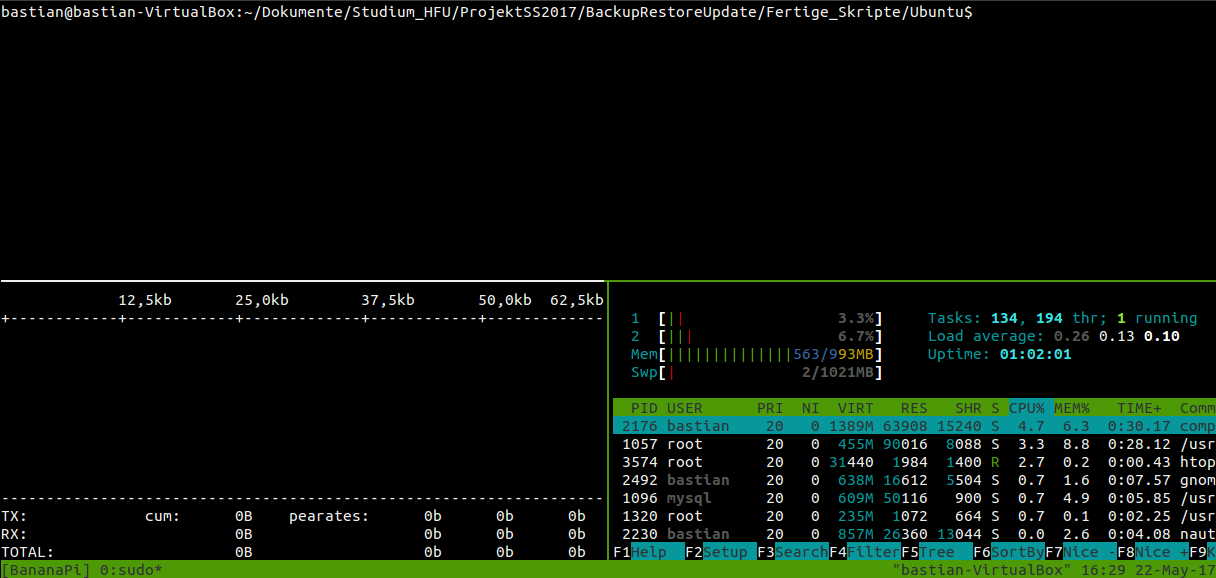
\includegraphics[width=\textwidth]{pictures/Bastian/Tmux}
\caption{Verwendung von Tmux mit 'htop' und 'iftop'}
\end{figure}

